\problemname{Rotating Mugs}

\illustration{0.3}{mugs.jpg}

At Lovable's office, they have some really cool coffee mugs. 
Despite having more sides in reality, we will model each mug as a simple object with four sides: \texttt{North}, \texttt{West}, \texttt{South}, and \texttt{East}.

You have $M$ mugs, indexed from $0$ to $M-1$, in front of you, 
and your task is to rotate the mugs so that the \texttt{North} side faces you. 
However, you may perform only \emph{magical rotations}. 
A magical rotation consists of the following three steps:
\begin{enumerate}
  \item Choose integers $a$ and $b$ such that $0 \le a < M$, $0 \le b < M-1$, and $a \neq b$. Note that $b$ cannot be the last index.
  \item Swap the mugs at indices $a$ and $b$ without rotating them.
  \item Take the mug now at index $b$ (the one moved from index $a$) and its neighbor to the right, then rotate both by $90^\circ$.
\end{enumerate}

When rotating a mug by $90^\circ$:
\begin{itemize}
  \item A mug with its \texttt{North} side facing you will now have its \texttt{West} side facing you.
  \item A mug with its \texttt{West} side facing you will now have its \texttt{South} side facing you.
  \item A mug with its \texttt{South} side facing you will now have its \texttt{East} side facing you.
  \item A mug with its \texttt{East} side facing you will now have its \texttt{North} side facing you.
\end{itemize}

You now wonder whether it is possible to arrange all the mugs so that their \texttt{North} sides face you using only magical rotations. To impress the task assigner, you would like to minimize the number of magical rotations.

If you do not have enough mugs on hand to experiment, you can use this \href{https://rotatingmugs.lovable.app/}{website}, created using Lovable, to simulate the magical rotations.
\section*{Input}
The first line contains an integer $M$ ($2 \leq M \leq 5 \cdot 10^5$), the number of cups infront of you.

The second line contains a string of $M$ characters $c_1, c_2, \dots, c_M$, where $c_i \in \{\texttt{``N''},\texttt{``W''},\texttt{``S''},\texttt{``E''}\}$ denotes the side of the $i$-th mug currently facing you.

\section*{Output}
Print a single integer: the minimum number of magical rotations required to make all mugs face the \texttt{North} side toward you. If it is impossible, print \texttt{-1}.

\section*{Scoring}
Your solution will be tested on a set of test groups, each worth a number of points. Each test group contains
a set of test cases. To get the points for a test group you need to solve all test cases in the test group.

\noindent
\begin{tabular}{| l | l | p{12cm} |}
  \hline
  \textbf{Group} & \textbf{Points} & \textbf{Constraints} \\ \hline
  $1$    & $25$       & From the start, all mugs either have their `North' or `East' side facing you. \\ \hline
  $2$    & $35$       & $M \leq 100$ \\ \hline
  $3$    & $40$       & No additional constraints. \\ \hline
\end{tabular}


\section*{Explanation of samples}
\noindent
In the first smaple, we start out with two mugs with initial state \texttt{WW}. 
By repeatedly choosing $a = 1$ and $b = 0$, the mugs will switch places and rotate $90^\circ$. Doing this 3 times, turns the mugs into the desired state. 
There exist no sequence of magical rotations that can achieve this in fewer than 3 moves.
\begin{figure}[h!]
  \centering
  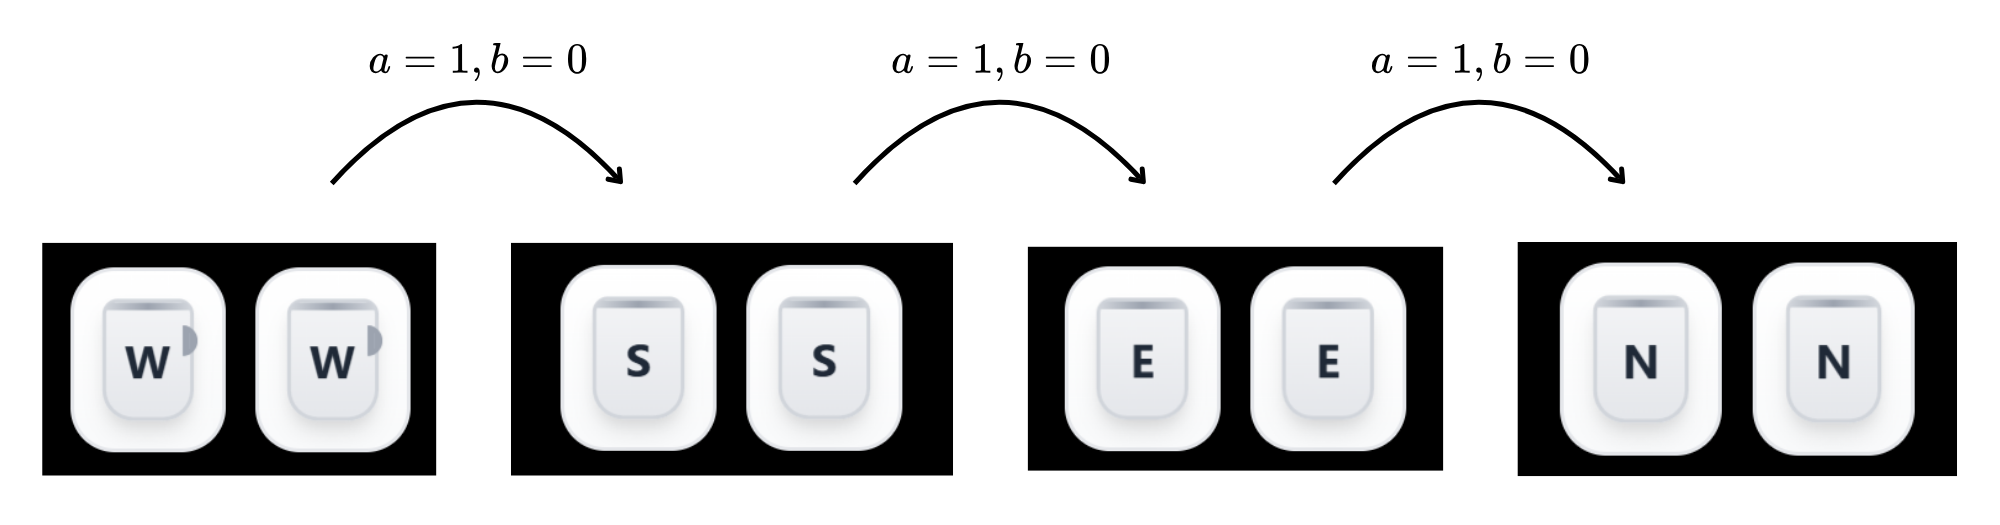
\includegraphics[width=0.5\textwidth]{sample1.png}
  \caption{Sequence of 3 magical rotations for sample 1.}
\end{figure}


\noindent
In the second sample, we start out with the mugs in the state \texttt{ESE}. We do the following two magical rotations:
\begin{itemize}
  \item Choosing $a = 2$, $b = 1$ will switch the positions of the mugs, leading to \texttt{EES}. Then we rotate the mugs now at position $b = 1$, and the one to the right of it by $90^\circ$, resulting in \texttt{ENE}.
  \item Choosing $a = 0$, $b = 1$ will switch the lead to \texttt{NEE}. Rotating the mug now at $b = 1$ and the one to the right of it results in \texttt{NNN}.
\end{itemize}
There exist no sequence of magical rotations that can achieve this in fewer than 2 moves.
\begin{figure}[h!]
  \centering
  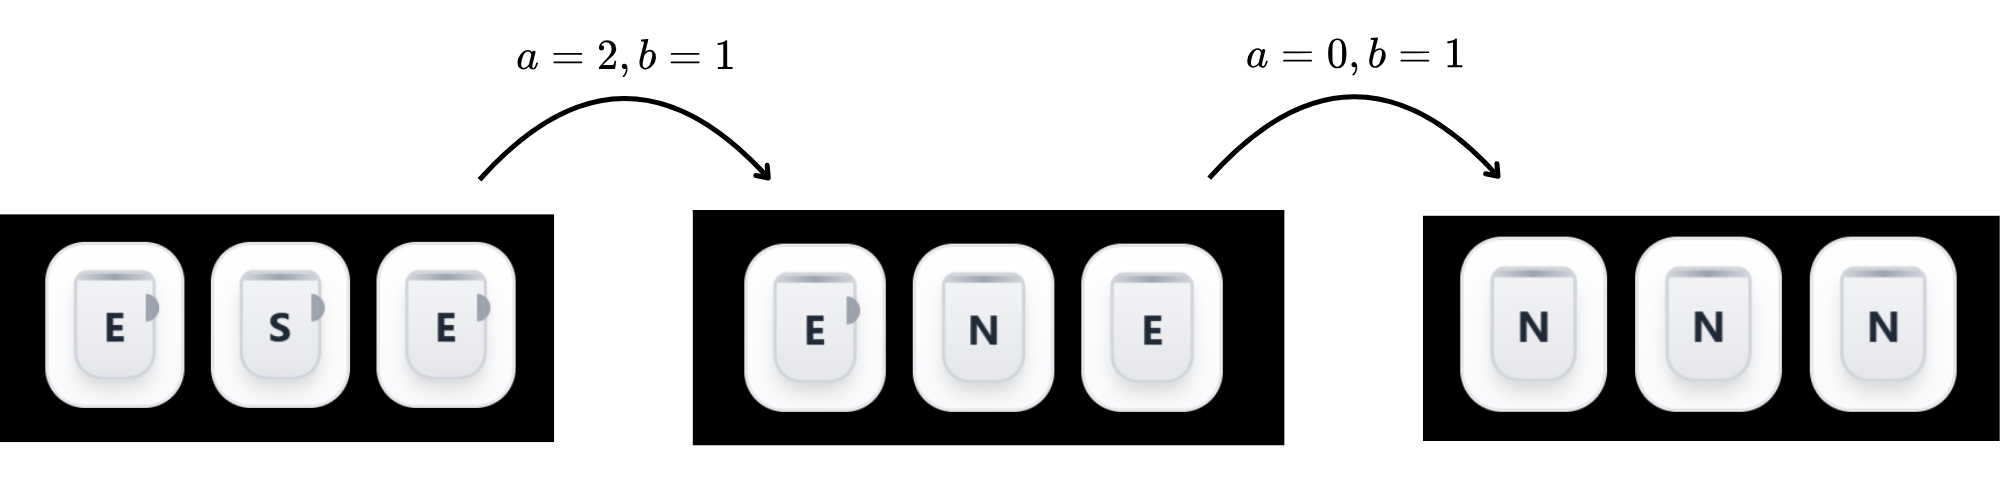
\includegraphics[width=0.5\textwidth]{sample2.png}
  \caption{Sequence of 2 magical rotations for sample 2.}
\end{figure}


\noindent
In the third sample, it can be proven that there exist no sequence of magical rotations that can turn all mugs such the mugs become \texttt{NNNNNN}. 